\chapter{Datenbank}\label{kap:Datenbank}
\section{Aufgabe der Datenbank}\label{kap:ZielDerDatenbank}
Die Datenbank soll den aktuellen Zustand der Produktionsanlage abbilden. Dazu gehören die Betriebsmittel, wie zum Beispiel die Fertigungs-Stationen oder die Roboter mit ihren aktuellen Status und der jeweiligen Ladung der Akkumulatoren. Es sollen auch die Verwaltungsdaten, wie Aufträge und Produktionsprozesse in der Datenbank gespeichert werden. Neben dem aktuellen Zustand der Produktionsanlage sollen auch die Fertigungsabläufe dort gespeichert werden. Dies beinhaltet in erster Linie eine Verfolgung der Werkstück durch Timestamps für das An- und Abmelden der Werkstück an den Bearbeitungs-Stationen. Es wird ebenso der Fortschritt, den ein Werkstück im Fertigungsprozess und ein Auftrag insgesamt gemacht hat, gespeichert. Eine weitere Aufgabe der Datenbank ist der Austausch von Daten zwischen dem Fertigungsrechner und der Fertigungsplanung. Alle Daten die zwischen diesen beiden Rechnern ausgetauscht werden, werden in die Datenbank geschrieben.
 
\section{Konzept} \label{kap:DatenbankKonzept}
Aus der realen Fertigungsanlage wird ein konzeptionelles Modell als Entität-Relation\-ship\--Diagramm modelliert. Das so modelliert ER-Diagramm ist in Abbildung \ref{fig:ER-Diagramm} zu sehen. Dazu werden insbesondere die Aufgaben aus Abschnitt \ref{kap:ZielDerDatenbank} berücksichtigt. Zur Qualitätssicherung wird sich an den drei gängigen Normalisierungsformen für Datenbanken orientiert. Anschließend wird das konzeptionelle Modell in ein logisches Datenschema überführt. Das Datenschema soll den Ansprüchen eines relationalen Datenbankmodells entsprechen. Zur Erstellung des Datenschemas wird die MySQL-Workbenche genutzt und deren Möglichkeit ein relationales Datenbankmodell grafisch zu entwerfen.
\begin{figure}[h]
	    \centering
	    \includegraphics[width=0.8\linewidth]{Bilder/ERChanDiagramm.png}
        \caption{Entität-Relationship-Diagramm}
        \label{fig:ER-Diagramm}
\end{figure}
 \section{Konzeptionelles Modell}
Zur Erstellung des konzeptionellen Modells wird für jede Betriebsmittelklasse der realen Anlage ein Entitätstyp angelegt. Es werden folgende Entitätstypen zur Repräsentation von Betriebsmitteln angelegt: Roboter, Arbeitsplatz, Parkplatz und Werkstück. Die vier Entitätstypen enthalten die zu speichernden Attribute der Betriebsmittel. So sollen für das Betriebsmittel Roboter zum Beispiel die Attribute \glqq Akkuleistung\grqq{}  und \glqq Status\grqq{}  gespeichert werden. Neben den Entitätstypen für die realen Betriebsmittel werden auch Entitätstypen für die Verwaltungsdaten, die zur Fertigungsplanung benötigt werden, angelegt. Hierzu zählen die Entitätstypen: Auftrag und Produktionsprozess. Der Entitätstyp Timestamp dient zur Speicherung der Fertigungsabläufe. Der Entitätstyp taggen dient ausschließlich zur Kommunikation zwischen der Fertigungsplanung und dem Programm für die Ansteuerung der RFID-Schreib-Lese-Köpfe. 

Zur Identifizierung der einzelnen Entitäten enthält jeder Entitätstyp mindestens ein Attribut oder eine Kombination von Attributen, die die Entitäten eindeutig unterscheiden. Viele der hier beschriebenen Entitätstypen haben ein aus der realen Welt abgeleitetes Attribut, wodurch die Entitäten unterschieden werden. So ist zum Beispiel die Roboter ID ein Wert der sich aus der Nummerierung der Roboter in der realen Welt ableitet. Es gibt allerdings auch Entitätstypen die eigentlich kein einzelnes Attribut haben, dass sie eindeutig unterscheidet. Als Beispiel hierfür kann der Timestamp genannt werden, wo sowohl der Zeitstempel als auch der Status einen Entität nicht eindeutig identifizieren. Erst in Kombination mit der Beziehung zu einem Werkstück kann der Zeitstempel die Entitäten eindeutig unterscheiden. Zur einfacheren Handhabung des Timestamps wird dem Entitätstyp ein zusätzliches Attribut \glqq id\_Timestamp\grqq{}  hinzugefügt. Dabei handelt es sich um eine laufende Nummer die keinen zusätzlichen Informationen speichert sondern nur der einfacheren Verwaltung dient. Die Attribute oder Kombinationen von Attributen die die Entitäten eines Entitätstyps eindeutig unterscheiden werden Schlüssel genannt. Wie schon beim Timestamp beschrieben, wurde darauf geachtet das jeder Entitätstype nur ein Attribut als Schlüssel hat.
 
Da die Betriebsmittel der realen Welt, ebenso wie die Daten der Fertigungsplanung oder die Fertigungsabläufe, in Beziehung zu einander stehen, werden die Entitätstypen mit Beziehungstypen verbunden und so die jeweilige Beziehung deutlich gemacht. Es gibt je nach Art der Beziehung verschiedene Beziehungstypen. Es werden Beziehungstyp-Richtungen mit Kardinalität 1 oder Kardinalität N verwendet. Wobei die Beziehungstyp-Richtungen mit der Kardinalität 1 sowohl optional als auch nicht-optional vorkommen. Alle vorkommenden Beziehungstypen sind in Tabelle \ref{tab:Beziehungstypen} aufgeführt. Die dort aufgeführten Beziehungen gelten natürlich umgekehrt genauso. Hat Auftrag zu Werkstueck eine 1:CN Beziehung, so hat Werkstueck zu Auftrag eine CN:1 Beziehung. Für die Beziehung zwischen einem Timestamp und einem Werkstueck bedeutet das zum Beispiel, dass ein Timestamp immer zu genau einem Werkstueck gehört, das Werkstueck aber keinen, einen oder mehrere Timestamps haben kann. Es sich also um einen 1:CN Beziehungstyp handelt. Ein Parkplatz hingegen kann immer nur für einen oder keinen Roboter reserviert sein. Genauso kann ein Roboter immer nur an einem oder an keinem Parkplatz sein. Es handelt sich also um eine C:C Beziehung. 

\begin{table}[htbp]
    \centering	
    \captionof{table}{Beziehungstypen}
    \begin{tabular}{|p{4cm}|p{8cm}|} 
    \hline Beziehungstyp &  zwischen  \cr 
    \hline \hline  C:C &  taggen zu werkstueck\newline roboter zu parkplatz \newline roboter zu werkstueck \cr
    \hline C1:CN  & arbeitsplatz zu roboter \newline arbeitsplatz zu werkstueck \cr
    \hline 1:CN  & werkstueck zu timestamp \newline arbeitsplatz zu timestamp \newline auftrag zu werkstueck \newline produktionsprozess zu werkstueck \cr
    \hline 
    \end{tabular}
    \newline
    \label{tab:Beziehungstypen}
\end{table}

Beim entwerfen des Datenmodells mit einem Entity-Relationship-Diagramm, gilt es verschiedene Punkte zu beachten. Besonders wichtig ist es, Redundanz bei Attributen zu vermeiden. Bei Redundanz treten verschiedene Probleme auf. So müssen die selben Daten mehrfach in die Datenbank geschrieben werden und es wird außerdem unnötig Speicherplatz belegt. Diese Probleme sind aufgrund der kleinen Datenmenge und der geringen Anzahl an Usern bei der hier beschriebenen Produktionsanlage wenig relevant. Redundanz ist auch deshalb zu vermeiden, weil sich ein Problem ergibt, wenn inkonsistente Daten entstehen, weil nicht an allen Stellen, die mehrfach vorhandenen Daten geändert wurden. Um Redundanzen in der Datenbank zu vermeiden, wird das Datenbankmodell normalisiert. Das Normalisieren ist im Abschnitt \ref{kap:Normalisierung} beschrieben.
Ebenso ist darauf zu achten keine, redundanten Beziehungstypen zu modellieren. Eine Redundanz kann immer dann vermutetet werden, wenn zwei Wege von einem Entitätstyp zu einem anderen Entitätstyp möglich sind. Beispielhaft sei hier der Entitätstyp Timestamp genannt, der sowohl eine direkte Beziehung zum Entitätstyp Werkstueck als auch eine indirekte Beziehung über den Entitätstyp Arbeitsplatz hat. Da es sich bei den beiden Beziehungen des Timestamps allerdings um zeitlich abgeschlossene Vorgänge handelt und die Beziehung zwischen Arbeitsplatz und Werkstück den aktuellen Zustand speichert, kann von der Beziehung des Timestamps zum Arbeitsplatz nicht auf das dazugehörige Werkstück geschlossen werden, so dass die direkte Beziehung zum Werkstück notwendig ist.\cite{Jarosch:2016}



\subsection{Normalisierung }\label{kap:Normalisierung}
Anhand von Normalisierungsstufen kann die Qualität eines Datenmodells beurteilt werden. Zur Qualitätssicherung wurden die ersten 3 Normalisierungsstufen auf das in Abschnitt \ref{kap:DatenbankKonzept} beschriebene und in Abbildung \ref{fig:ER-Diagramm} dargestellte konzeptionelle Datenmodell angewandt. Durch die Anwendung der 3 Normalisierungsstufen entsteht ein Datenmodell, dass in der 3. Normalform vorliegt. Das Vorliegen in der 3. Normalform bietet auch bei der Überführung in das relationale Datenbank-Modell Vorteile Beziehungsweise ist bei Stufe 1 sogar Voraussetzung.

\subsubsection*{1. Normalform}
Die erste Normalform besagt das eine Entität keine Attribute besitzen darf die zur gleichen Zeit mehrere Werte annehmen können. So würde es zum Beispiel gegen die 1. Normalform verstoßen wenn die Zeitstempel als Attribut des Werkstücks angelegt worden wären, da dieses Attribut, je nach dem wie viele Stationen das Werkstück schon durchlaufen hat, mehrere Werte annehmen könnte. Um die 1. Normalform zu erreichen, werden Attribute die mehrere Werte annehmen können aus dem Entitätstyp herausgelöst und bilden einen eigenen Entitätstyp, der durch einen Beziehungstyp mit dem ursprünglichen Entitätstyp verbunden ist. Dabei hat die Beziehungstyp-Richtung "`Ursprüngliche Entitätstyp zu neuem Entitätstyp"' die Kardinalität N oder CN.
Angewandt auf das Beispiel des Zeitstempels wurde, wie in Abbildung \ref{fig:ER-Diagramm} zu sehen ist, der Zeitstempel in den neuen Entitätstype Timestamp ausgelagert. Der Beziehungstyp-Richtung von Werkstück zu Timestamp ist CN.
Ein Wert welcher nicht aus einer Liste besteht oder auf andere Weise aus mehreren Werten zusammengesetzt ist wir als atomarer Wert bezeichnet. Für ein relationales Datenbank-Modell gilt: Jeder Wert eines Attributes muss ein atomarer Wert sein.\cite{Jarosch:2016}

\subsubsection*{2. Normalform}
Damit ein Datenmodell in der 2. Normalform vorliegt, muss es sich in der ersten Normalform befinden. Zusätzlich darf jedes Attribut ausschließlich vom Gesamtschlüssel eines Entitätstyps funktional Abhängig sein. Funktionale Abhängigkeit bedeutet, dass aus dem Wert von Attribut A sich automatisch der Wert von Attribut B ergibt. Zum Verdeutlichen der zweiten Normalform nutze ich ein etwas konstruiertes Beispiel: Angenommen die Produktionsanlage fährt mit zwei verschiedenen Typen von Robotern. Mit jeweils zwei alten Festo-Robotern und zwei neuen von Studenten entwickelten Robotern. Die ID der Roboter setzt sich nun aus zwei Ziffern zusammen die jeweils ein eigenes Attribut bilden und zusammen den Gesamtschlüssel für den Entitätstyp Roboter. Die erste Ziffer wäre dabei entweder eine 1 für die Festo-Roboter oder eine zwei für die neuen Roboter. Die zweite Ziffer ist eine laufende Nummer. Wird jetzt zusätzlich das Baujahr gespeichert und sind die Roboter eines Typs jeweils im gleichen Jahr gebaut so liegt eine funktionale Abhängigkeit zwischen dem Attribut Baujahr und dem Teilschlüssel erste Ziffer vor. Um die zweite Normalform nun herzustellen wird der Teilschlüssel und das abhängige Attribut herausgelöst und sie bilden einen neuen Entitätstyp. Die zweite Normalform verringert Redundanzen innerhalb des Datenmodells.\cite{Heuer:2001}

\subsubsection*{3. Normalform}
Damit ein Datenmodell in der 3. Normalform vorliegt muss es sich in der 2. Normalform befinden und zusätzlich darf eine Attribut eines Entitätstyps nicht transitiv funktional abhängig sein.  So wäre es zum Beispiel möglich, die Attribute des Entitätstyps Produktionsprozesses mit im Entitätstyps Werkstück zu speichern. Es läge dann allerdings eine transitive funktionale Abhängigkeit zwischen den Werten der Attribute Station 1 bis 5 und Dauer Station 1 bis 5 und dem Schlüssel RFID Werkstück vor, da die Attribute Station 1 bis 5 und Dauer Station 1 bis 5 funktional von der id\_Produktionsprozess abhängig wären. Die id\_Produktionsprozess wiederum wäre funktional abhängig vom Schlüssel RFID Werkstück. Deshalb wird dieser Teil herausgelöst und bildet einen eigenen Entitätstyp. Die dritte Normalform verringert die Gefahr von Redundanzen im Datenmodell.\cite{Heuer:2001}

\section{Relationales Datenbankmodell}\label{kap:relationales_Datenbankmodell}
Bei einer MySQL-Datenbank handelt es sich um eine relationale Datenbank. Dabei entspricht eine Entität aus dem ER-Diagramm einem Tupel von Werten und der Entitätstyp einem Relationstyp. 

So lässt sich nun die Mengen aller Entitäten eines Entitätstyps als Tabelle darstellen. Dabei entsprechen die Überschriften der einzelnen Spalten den Namen der Attribute. Was im ER-Diagramm Attribute genannt wurde, wird nun Eigenschaften genannt. Eine Zeile repräsentiert dann jeweils eine Entität Beziehungsweise ein Tupel von Werten. Wie schon beim ER-Diagramm hat jeder Relationstyp ein oder mehrere Attribute zur eindeutigen Identifizierung der jeweiligen Tupel, die im relationalen Datenbankmodell als Primärschlüssel bezeichnet werden und dem Schlüssel im ER-Diagramm entsprechen. Beziehungstypen werden über sogenannte Fremdschlüssel realisiert. Fremdschlüssel stellen eine zusätzliche Spalte in einer Tabelle da. Ist in einer Tabelle ein Fremdschlüssel eingetragen, referenziert dieser auf eine  Zeile einer anderen Tabelle und stellt so die Beziehung her. Dabei muss stets die referenzielle Integrität dieser Verweise gewährleistet sein, dass bedeutet das ein Fremdschlüssel immer auf eine vorhandene Zeile einer anderen Tabelle referenzieren muss oder mit einem NULL-Marker belegt sein muss. 

\section{Zugriff auf die Datenbank}\label{kap:DatenbankZugriff}
Die MySQL-Datenbank ist auf einem Server, der auf dem Fertigungsrechner läuft, implementiert. Es gibt zwei User die Zugriff auf die Datenbank benötigen. Das ist zum einen die Fertigungsüberwachung, die das Auslesen der RFID-Tags übernimmt und die Fertigungsplanung. Die Fertigungsüberwachung befindet sich auf dem selben Rechner wie der Server der Datenbank. Die Fertigungsplanung ist auf einem anderen Rechner realisiert und über Ethernet mit dem Fertigungsrechner verbunden. Die Fertigungsplanung ist mit Qt ausgeführt und hat über eine eingebundene Bibliothek über Ethernet direkten Zugriff auf die Datenbank. 

Die Fertigungsüberwachung läuft auf einer Soft-SPS auf dem Fertigungsrechner und ist mit CODESYS programmiert. Ein direkter Zugriff von der Soft-SPS auf die Datenbank ist nicht möglich. Ein Zugriff könnte über einen OPC-Server erfolgen. OPC (Open Platform Communications) ist eine standardisierte Softwareschnittstelle. Sie ermöglicht den Datenaustausch zwischen Steuerungen verschiedener Hersteller aus der Automatisierungstechnik. Hier wurde allerdings ein anderes Verfahren, speziell für den Zugriff auf Datenbanken von Steuerungen aus der Automatisierungstechnik, angewandt. Es handelt sich dabei um den SQL4Automation Connector der Firma Inasoft Systems GmbH. Dieser wurde speziell für den Zugriff von Speicherprogramierbaren Steuerungen auf eine Datenbank entwickelt und ermöglicht sowohl Lese- als auch Schreibbefehle in SQL direkt auf der SPS zu programmieren. Für die verwendete Steuerung ist schon eine fertige Bibliothek vorhanden, was die Anwendung deutlich erleichtert. In Abbildung \ref{fig:DatenbankZugriffUebersicht} ist schematisch dargestellt, wie auf die Datenbank zugegriffen wird.

\begin{figure}[ht]
	    \centering
	    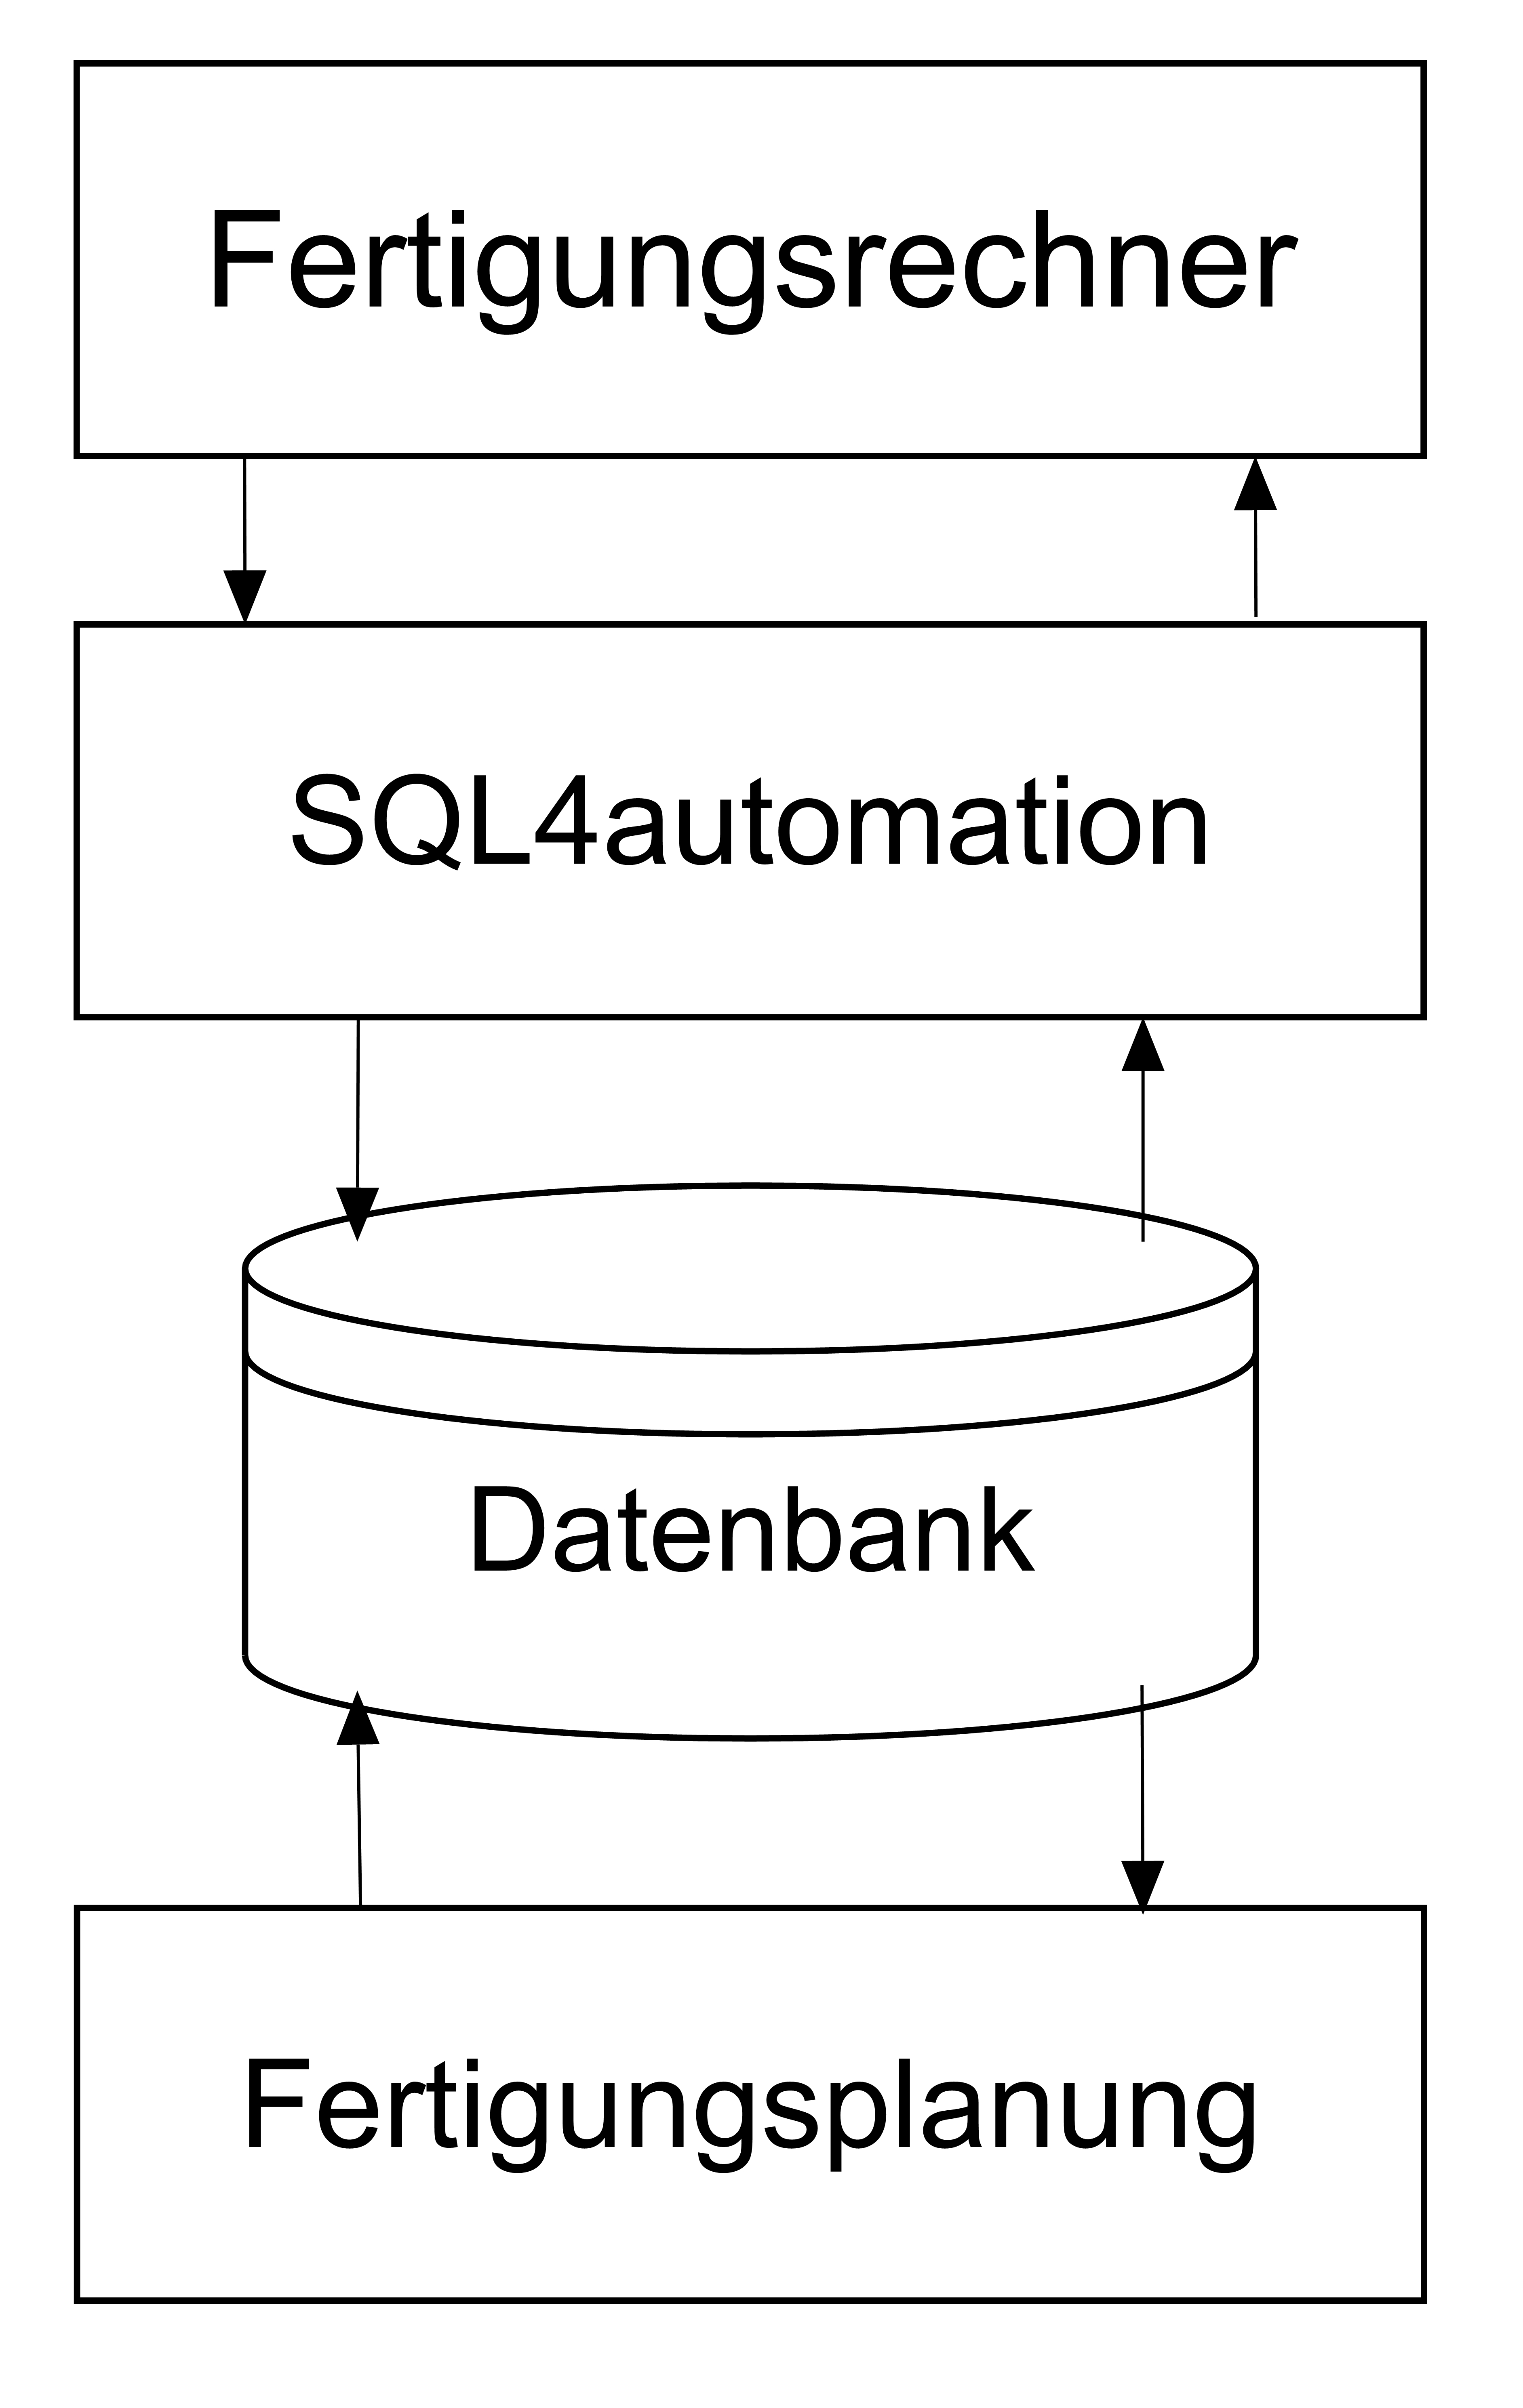
\includegraphics[width=0.4\linewidth]{Bilder/Datenbankdiagramm.png}
        \caption{Schematische Darstellung des Datenbankzugriffs}
        \label{fig:DatenbankZugriffUebersicht}
\end{figure}


\section{Umsetzung des entwickelten Modells}
Zunächst wurde anhand des in Abschnitt \ref{kap:DatenbankKonzept} beschriebenen Konzeptes das ER-\-Dia\-gramm der Datenbank grafisch entwickelt. Das so entstandene ER-Diagramm, ist in Abbildung \ref{fig:ER-Diagramm} zu sehen. Die Entwicklung des ER-Diagramms erfolgte in enger Absprache mit der Fertigungsplanung, da diese einer von zwei Nutzern der Datenbank ist.
 
\begin{figure}[ht]
	    \centering
	    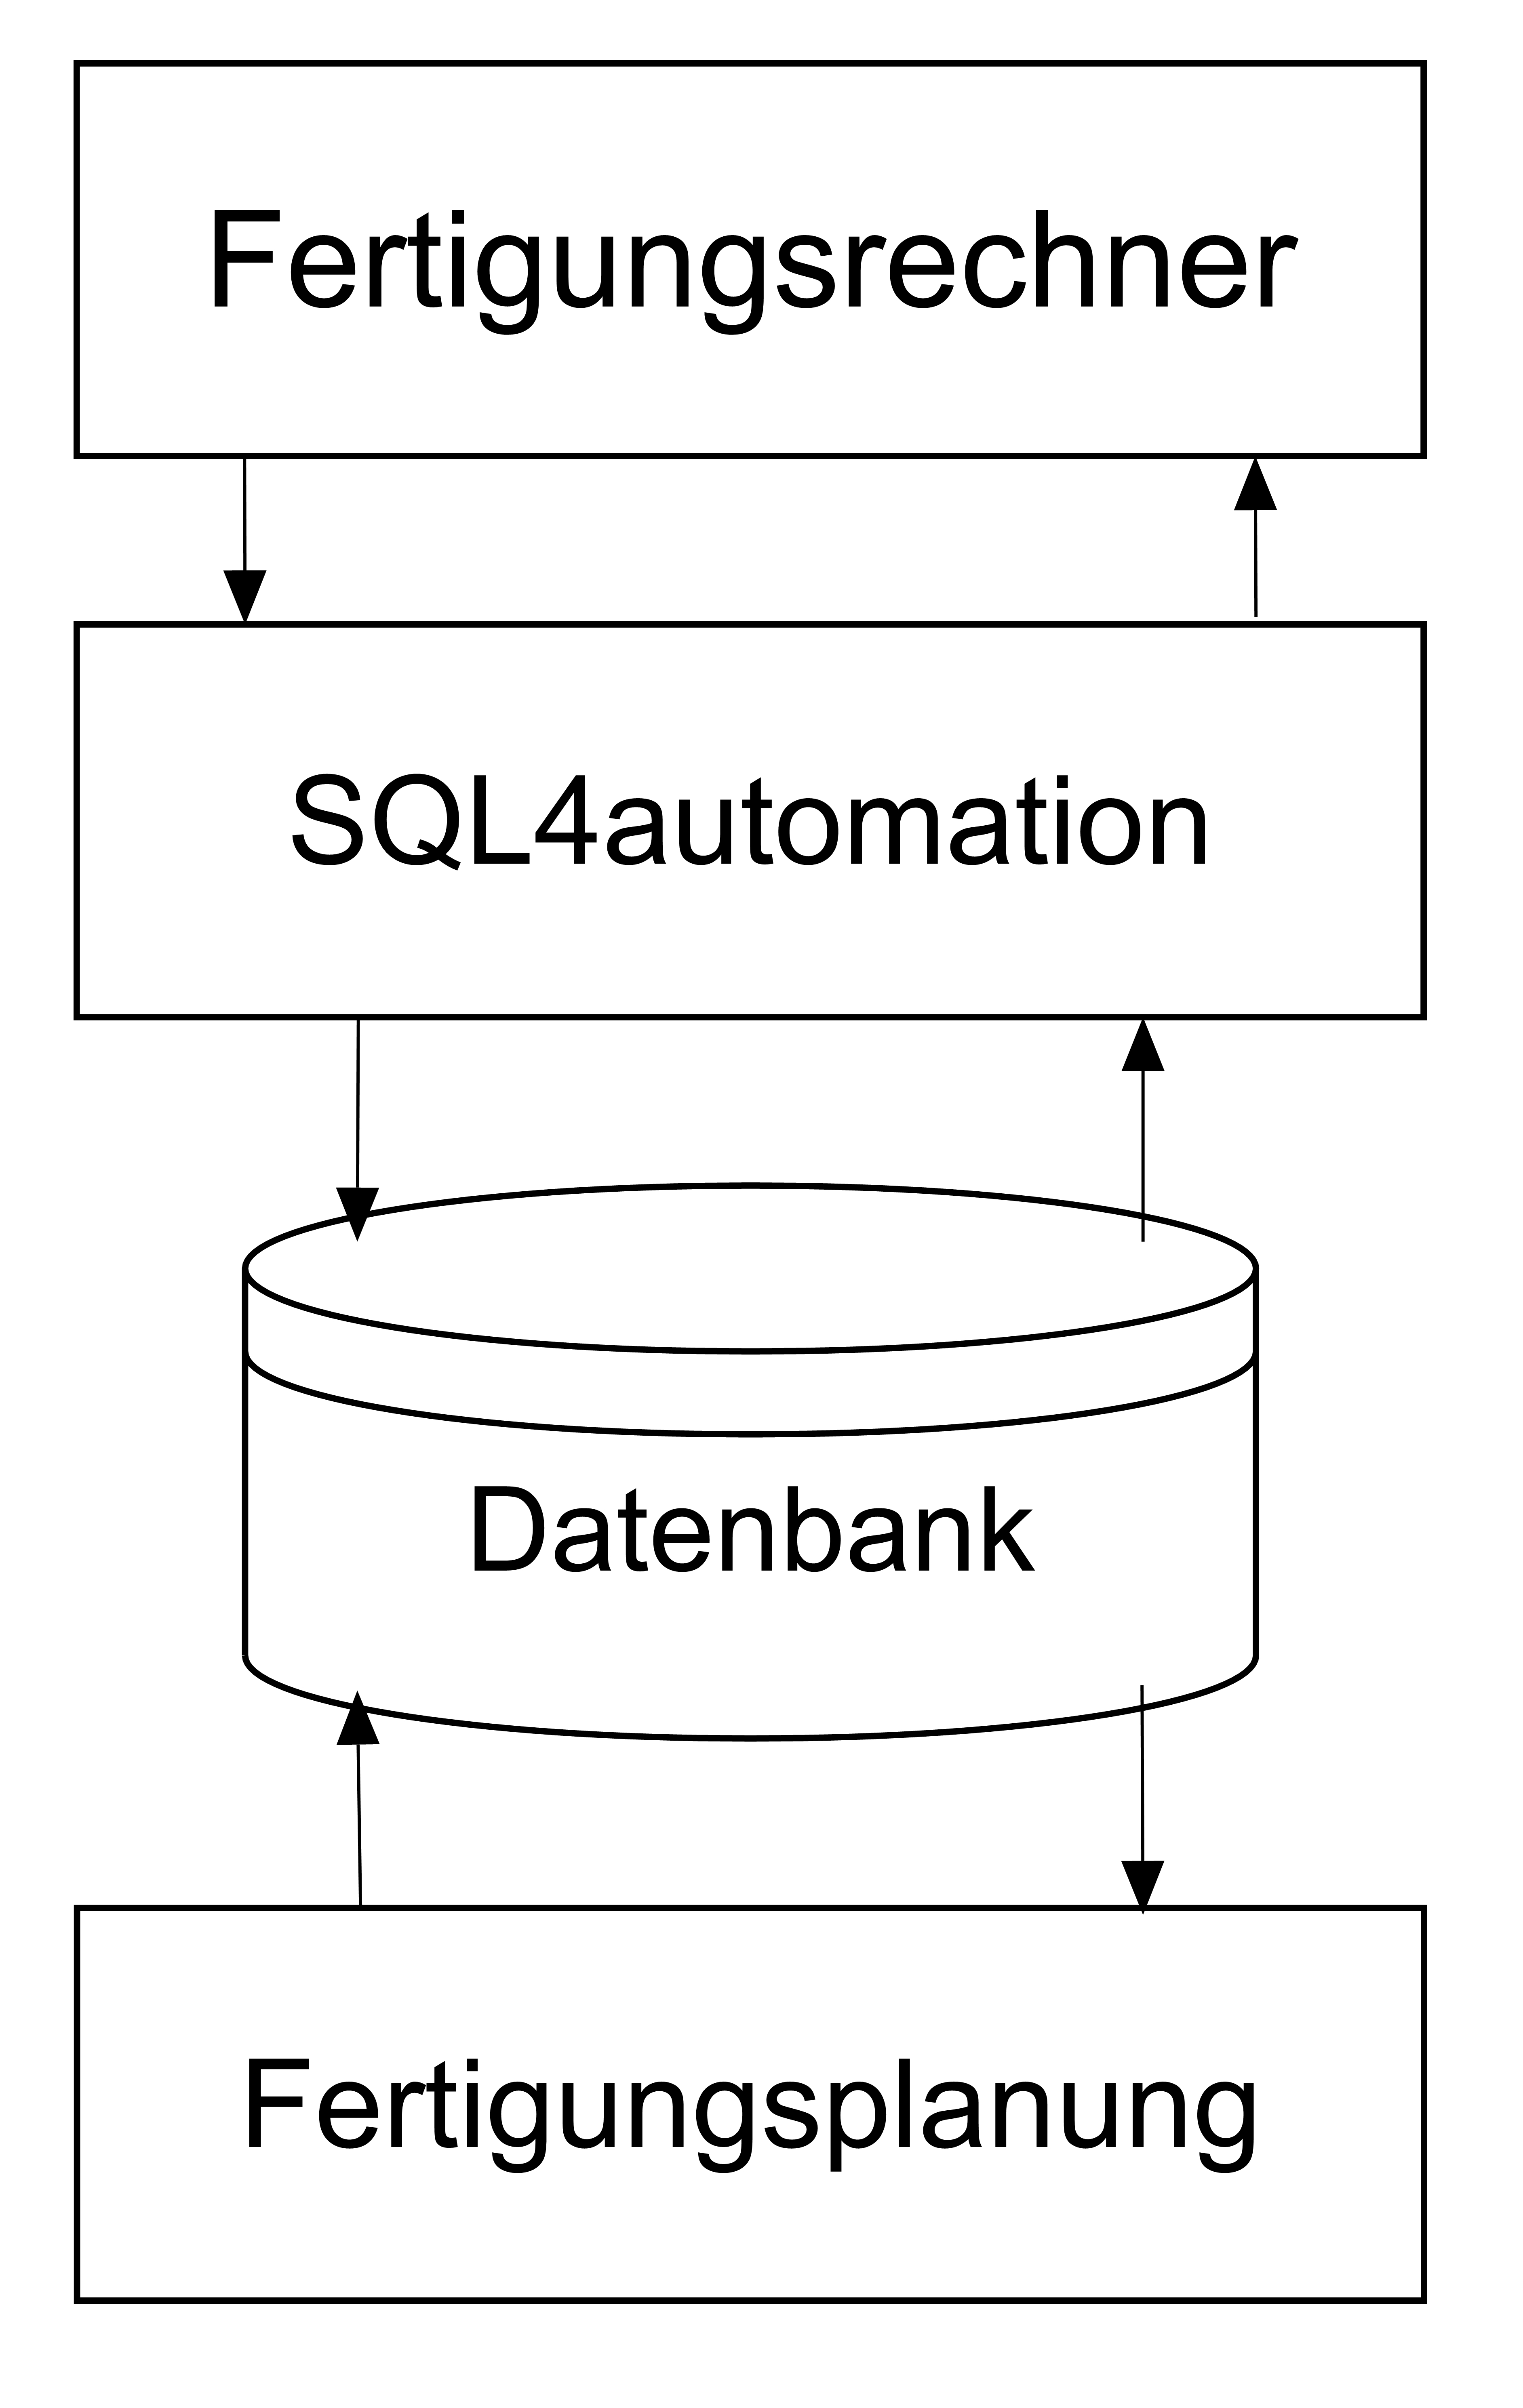
\includegraphics[width=0.4\linewidth]{Bilder/Datenbankdiagramm.png}
        \caption{Grafisches Modell der Datenbank}
        \label{fig:ER-Diagramm_Worbenche}
\end{figure}
 
Zum Erstellen der Datenbank wurde das Tool MySQL-Workbenche vom Entwickler Oracle Corporation genutzt. Dieses Tool ermöglicht die visuelle Entwicklung, Erstellung und Bearbeitung einer Datenbank. Es können außerdem MySQL-Befehle, zum Beispiel zum Testen, ausgeführt werden. Die visuelle Entwicklung erfolgt über die grafische Eingabe des aus dem ER-Diagramm entwickelten relationalen Datenbankmodells wie in Abbildung \ref{fig:ER-Diagramm_Worbenche} dargestellt. In der Tabelle \ref{tab:ER-Erklaerung} sind die Symbole, die durch die MySQL-Workbenche verwendet werden, beschrieben.
%\begin{comment}
\begin{table}[ht]%{1\textwidth}
    \centering	
			\renewcommand{\arraystretch}{2}

    \captionof{table}{Zeichenelegende MySQL-Workbench Modell}
    \begin{tabular}{|p{1.8cm}|p{8cm}|} 

    \hline Zeichen &  Bedeutung  \cr 
    \hline \hline   
\includegraphics[width=0.5cm,]{Bilder/ER/Primaerschluessel.PNG} &  Primärschlüssel \cr
    \hline 
\includegraphics[width=0.5cm,]{Bilder/ER/EigenschaftNN.PNG}  & Eigenschaft (darf nicht NULL sein) \cr
    \hline 
\includegraphics[width=0.5cm,]{Bilder/ER/Eigenschaft.PNG}  & Eigenschaft \cr
    \hline 
\includegraphics[width=0.5cm,]{Bilder/ER/FremdschluesselNN.PNG}  &  Fremdschlüssel (darf nicht NULL sein)\cr
    \hline 
\includegraphics[width=0.5cm,]{Bilder/ER/Fremdschluessel.PNG}  & Fremdschlüssel \cr
    \hline 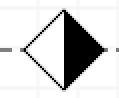
\includegraphics[width=0.5cm,]{Bilder/ER/1zuN.PNG}  & 1:N Beziehung \cr 
    \hline 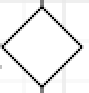
\includegraphics[width=0.5cm,]{Bilder/ER/1zu1.PNG} &  1:1 Beziehung \cr
    \hline 
    \end{tabular}
    \newline
    \label{tab:ER-Erklaerung}
\end{table}
%\end{comment}
Es können dort die Entitätstypen, welche in das relationale Datenbankmodell transformiert einer Tabelle entsprechen, angelegt werden. Jeder Tabelle können ein Primärschlüssel und Eigenschaften zugewiesen werden. Sowohl dem Primärschlüssel, als auch den Eigenschaften muss ein Datentyp zugewiesen werden. Es können auch weitere Festlegungen für die Eigenschaften getroffen werden. So kann eine Eigenschaft als \glqq NOT NULL\grqq{}  festgelegt werden, was bedeutet, dass beim Anlegen einer neuen Entität beziehungsweise einer neuen Zeile in der Tabelle diese Eigenschaft immer gesetzt werden muss und auch nicht später gelöscht werden kann. So muss zum Beispiel ein Parkplatz immer einen Status haben. Beim Produktionsprozess, der nicht immer die selbe Länge hat, ist es nicht notwendig das alle Eigenschaften immer einen Wert haben. So brauch ein Produktionsprozess mit nur 4 Stationen die Eigenschaften \glqq station\_5\grqq{}  und \glqq dauer\_station\_5\grqq{}  nicht. Der Primärschlüssel muss selbstverständlich immer vergeben werden und darf nicht mit einem  NULL-Marker belegt sein.
Auch Beziehungstypen können in der MySQL-Workbenche abgebildet werden. Wird ein Beziehungstyp angelegt, so erzeugt dieser automatisch den, wie in Abschnitt \ref{kap:relationales_Datenbankmodell} beschrieben, dazugehörigen Fremdschlüssel in den jeweiligen Tabellen. Je nach Beziehungstyp dürfen diese durch einen NULL-Marker belegt  sein oder müssen eine Wert haben. So kann bei einer optionalen C1:CN Beziehung, wie sie zum Beispiel von Arbeitsplatz zu Roboter besteht, das Feld für den Fremdschlüssel auch \glqq NULL\grqq{}  sein. Bei einer 1:CN Beziehung, wie vom Auftrag zum Werkstueck, darf der Fremdschlüssel \glqq auftrag\_id\_auftrag\grqq{}  beim Werkstück nicht mit einem NULL-Marker belegt sein, da jedes Werkstück einem Auftrag zugeordnet werden muss.
 
Nach dem grafischen Entwurf der Datenbank kann mittels der Option \glqq Forward Engineer to Database\grqq{}  aus dem grafischen Modell automatisch der entsprechende Code für die Datenbank erstellt werden und die Datenbank ohne weitere Programmierung implementiert werden. Auch nachträgliche Änderungen oder Erweiterungen an der Datenbank können direkt im grafischen Modell erfolgen und über die \glqq Forward Engineer to Database\grqq{}  Option direkt eingepflegt werden. So bleibt das grafische Modell und die Datenbank immer auf dem selben Stand. Es ist keine zusätzliche Pflege der Dokumentation während des Entwicklungsprozess nötig. 
 
Nach dem Erstellen der Datenbank lässt sich die Struktur der Datenbank im Navigator der MySQL-Workbenche betrachten. Zum Befüllen der Datenbank lassen sich über das Abfragefenster MySQL-Befehle, wie zum Beispiel \glqq INSERT INTO\grqq{},  ausführen. Beim Befüllen ist insbesondere darauf zu achten, die Tabellen in der richtigen Reihenfolge zu befüllen. So kann ein Werkstück zum Beispiel erst angelegt werden, wenn der dazugehörige Auftrag bereits erstellt wurde.
 
Über das Abfragefenster lassen sich auch die MySQL-Befehle, die später im CODE\-SYS-Programm auf der Soft-SPS sowie im mit Qt entwickelten Programm auf dem Fertigungsrechner implementiert werden, testen. Auf die MySQL-Befehle die für Qt entwickelt wurden wird in \ref{kap:MySQLBefehle} eingegangen. 

Das Erstellen der MySQL-Befehle lief nach und nach parallel zur Entwicklung der beiden User-Programme der Datenbank. Zunächst wurde die Anforderung an den Befehl festgelegt. Anschließend wurde der Befehl erstellt und mit der MySQL-Workbenche getestet. Nach dem erfogreichen Test wurde der Befehl in seine Zielumgebung, also CODESYS oder Qt, portiert und dort erneut getestet. Beim Testen der Befehle ist insbesondere der Error-Code interessant. Er liefert wichtige Hinweise warum ein Befehl nicht funktioniert. Der Error-Code kann anhand von Error-Code Listen dekodiert werden. Für die Tests in der MySQL-Workbenche übernimmt das dekodieren die Entwicklungsumgebung.

\section{MySQL-Befehle für die Fertigungsplanung}\label{kap:MySQLBefehle}
Im folgenden Abschnitt wird zunächst allgemein beschrieben wie die in Qt verwendeten MySQL-Befehle aufgebaut sind und anschließend jeweils ein Befehl der drei Klassen Getter, Setter und Update näher beschrieben. Hier wird nur auf den Aufbau der MySQL-Befehle eingegangen. Wie der Aufruf der Funktion aus Qt heraus funktioniert ist in Abschnitt \ref{sec:Databasehandler} beschrieben.

Es hat sich für die Implementierung in Qt herausgestellt, dass es sinnvoll ist zunächst mit einem SET-Befehl eine Variable zu deklarieren und ihr einen Wert zuzuweisen. Das erhöht die Lesbarkeit des Codes, da die eigentliche Abfrage nicht zerschnitten werden muss. 
\subsection{Getter}\label{kap:MySQLGetter}
Im Folgenden wird beispielhaft ein MySQL-Befehl aus einem Getter in Qt beschrieben: Ein Getter fragt Werte aus der Datenbank ab, ohne diese zu verändern.
Im Listing \ref{lst:MySQLQtGetter} ist der Code für die Abfrage, ob und welcher Arbeitsplatz an einer Station frei ist, dargestellt. Der Befehl befindet sich in der Funktion GetZielStationsplatzFree(int Station). Die Zuweisung zur Variable \glqq @Station1\grqq{} entspricht dabei dem der Funktion übergebenen Wert mit 10 multipliziert, da die einzelnen Plätze wie in Abbildung \ref{fig:Positionskodierung} dargestellt kodiert sind. Diese Abfrage liefert eine 1 zurück wenn beide (Zeile 4) oder der erste (Zeile 5) Arbeitsplatz der entsprechenden Station frei sein. Ist nur der zweite Arbeitsplatz frei liefert die Abfrage eine 2 (Zeile 6) und sollten alle Arbeitsplätze belegt sein, wird eine 0 zurückgeliefert (Zeile 7).
 
\lstset{ 
    keywordstyle        =\bfseries\ttfamily\color{blue},
    basicstyle          =\scriptsize\ttfamily, 
    emphstyle           =\color{red},
    %identifierstyle     =\color{magenta},
    numbers             =left,
    xleftmargin         =15pt,
    backgroundcolor     =\color{newgray},
    showstringspaces    =false,
    language            =SQL
    }	 

\begin{lstlisting}[caption={MySQL-Befehl: Freier Arbeitsplatz }
       \label{lst:MySQLQtGetter}, float=hbt,
       captionpos=t] 
SET @Station1 = station*10; 
SELECT
    (CASE
        WHEN(SUM(id_Arbeitsplatz))=@Station1+1+@Station1+2 THEN 1 
        WHEN(SUM(id_Arbeitsplatz))=@Station1+1 THEN 1 
        WHEN(SUM(id_Arbeitsplatz))=@Station1+2 THEN 2 
        ELSE 0 
    END) 
FROM 
    vpj.arbeitsplatz 
WHERE (id_Arbeitsplatz IN (@Station1+1,@Station1+2) 
        AND Werkstueck_RFID_Werkstueck is NULL);
\end{lstlisting}

Bei den MySQL-Gettern handelt es sich meistens um Abfragen die nur einen Wert zurück liefern und keine ganzen Tabellen, so dass die Rückgabewerte direkt eine Aussage treffen und nicht die  Tabellen erneut durchsucht werden müssen. Ziel war es, die Abfragen so präzise wie möglich zu gestalten, um die Nachbearbeitung der Abfrage-Ergebnisse weitestgehend zu verhindern. Eine Ausnahme stellen hierbei die Daten da die später als Listen in der Visualisierung ausgegeben werden. Beispielhaft seien hier die RFID-Timestamps mit den dazugehörigen Zeiten und Arbeitsplätzen genannt, die als Liste zurückgegeben werden.

\subsection{Update}\label{kap:MySQLUpdate}
Im Folgenden wird beispielhaft ein MySQL-Befehl aus einer Update-Funktion in Qt beschrieben: Eine Update-Funktion verändert einen vorhandenen Eintrag in der Datenbank. Im Listing \ref{lst:MySQLQtUpdate} ist der MySQL-Befehl der Funktion UpdateParkplatz(int ID, int status, int roboterid) dargestellt. Mit dieser Funktion kann einem Parkplatz in der Datenbank ein neuer Roboter sowie ein neuer Status zugewiesen werden. Wie auch beim Getter werden die Variablen zunächst mit einem Set-Befehl gesetzt. Wenn ein Roboter einen Parkplatz nicht mehr belegt, muss das Feld Roboter\_id\_Roboter auf NULL gesetzt werden. Da im Funktionskopf nur ein Integer übergeben wird, wird über eine if-else-Abfrage die Variable @robo auf NULL gesetzt, wenn die, an die Funktion übergebene roboterid 0 ist.
Nach dem Setzen der Variablen (Zeile 1-3) wird in Zeile 4 festgelegt welche Tabelle ein Update erfahren soll. Mit dem Set-Befehl aus Zeile 5 werden die beiden Felder aus Zeile 6 und 7 überschrieben. Dabei wird beim Überschreiben des Fremdschlüssels Roboter\_id\_Roboter die Beziehung eines Roboters zu einem Parkplatz geändert oder gekappt. In Zeile 8 und 9 wird über den Primärschlüssel ausgewählt, welche Zeile der Tabelle ein Update bekommt.

\begin{lstlisting}[caption={MySQL-Befehl: Update Parkplatz }
       \label{lst:MySQLQtUpdate}, float=hbt,
       captionpos=t]
SET @Parkplatz=ID;
SET @Status=status;
SET @robo=roboterid;
UPDATE vpj.parkplatz
SET 
    Status=@Status, 
    Roboter_id_Roboter=@robo 
WHERE 
    id_Parkplatz=@Parkplatz;
\end{lstlisting}
Die Update Funktionen werden insbesondere für Tabellen genutzt in denen eine feste, durch die reale Welt vorgegebene, Anzahl an Zeilen vorhanden ist. Also zum Beispiel die Roboter. Die Roboter werden nicht mehr oder weniger, es ändern sich allerdings die einzelnen Werte der Eigenschaften.

\subsection{Setter}\label{kap:MySQLSetter}
Im Folgenden wird beispielhaft ein MySQL-Befehl aus einer Setter-Funktion in Qt beschrieben: Eine Setter-Funktion erzeugt einen neuen Eintrag in der Datenbank. Das Listing \ref{lst:MySQLQtSetter} enthält die MySQL-Befehle zum Anlegen eines neuen Auftrags in der Datenbank und den dazugehörigen Werkstücken. Mit der Abfrage in den Zeilen 1-4 wird die höchste Auftrags ID ermittelt, damit der nächste Auftrag die nächst höhere ID bekommt und es keine Konflikte bei den Primärschlüsseln gibt. Mit dem INSERT INTO Befehl aus Zeile 5 wird eine neue Zeile in der Tabelle vpj.auftrag angelegt. Die Zeile erhält die Werte aus Zeile 8. Mit dem Befehl aus Zeile 9-12, wird nun eine neues Werkstück angelegt und über das Feld auftrag\_id\_auftrag mit dem Auftrag verknüpft. Da das Feld auftrag\_id\_auftrag nicht NULL sein darf, muss, bevor ein Werkstück in die Datenbank geschrieben wurde, immer erst der entsprechende Auftrag angelegt werden. 

\lstset{ 
    keywordstyle        =\bfseries\ttfamily\color{blue},
    basicstyle          =\scriptsize\ttfamily, 
    emphstyle           =\color{red},
    %identifierstyle     =\color{magenta},
    numbers             =left,
    xleftmargin         =15pt,
    backgroundcolor     =\color{newgray},
    showstringspaces    =false,
    language            =SQL
    }	 


\begin{lstlisting}[caption={MySQL-Befehl: Update Parkplatz }
       \label{lst:MySQLQtSetter},float=tbh,
       captionpos=t]
SELECT
    MAX(id_auftrag)
FROM
    vpj.auftrag;
INSERT INTO
    vpj.Auftrag
VALUES 
    (maxID, 0);
INSERT INTO
    vpj.Werkstueck 
VALUES 
    (werkstueck, 0, produktionsprozess, maxID);
\end{lstlisting}
Die Setter werden insbesondere für die Tabellen mit dynamischer Größe genutzt. Beispielhaft sei hier die Tabelle mit den Aufträgen genannt, die während der Programmlaufzeit die ganze Zeit über erweitert werden kann. Die Setter werden auch zu Programmstart genutzt, um die Datenbank initial zu befüllen.